% PLAYGROUND — a toy document for trying out the thesis setup.
% Nothing here is part of the thesis. Break it, change it, learn from it.
% It uses the thesis's own preamble (../config/preamble.tex), so whatever
% works here works in the thesis.

\documentclass[a4paper, 10pt, oneside]{report}

% Author notes on; \workingdraftfalse hides them all.
\newif\ifworkingdraft
\workingdrafttrue

\input{preamble}
\addbibresource{references.bib}

\DeclareAcronym{tp}{short = TP, long = temperatura pokojowa}
\DeclareAcronym{bpm}{short = BPM, long = bulgotanie na minutę}

\title{Rosół według przepisu babci\\\large dokument do zabawy szablonem}
\author{Zespół kuchenny}
\date{\today}

\begin{document}

\maketitle
\tableofcontents

\chapter*{Wykaz skrótów}
\addcontentsline{toc}{chapter}{Wykaz skrótów}
\printacronyms[heading=none]

% !TeX root = ../main.tex
\chapter{Wstęp}
\label{chap:introduction}

% One sentence per line: the PDF still shows one paragraph, but a git diff
% shows exactly which sentence changed. An empty line starts a new paragraph.
Rosół jest zupą, o której każda babcia ma własne zdanie~\cite{babcia1987zupy}.
W niniejszym dokumencie przedstawiono przepis sprawdzony w wielu niedzielnych obiadach.
Celem pracy jest pokazanie, że przygotowanie rosołu da się opisać tak samo starannie jak system przetwarzania strumieniowego~\cite{kuchcik2021bulion, garnek2019teoria}.

\section{Motywacja}
\label{sec:motivation}

Rosół gotuje się wolno -- to jego zaleta, a nie wada.
Cytaty zapisuje się poleceniem \code{\\enquote}, które daje polskie cudzysłowy: \enquote{nie ma pośpiechu przy rosole}~\cite[s.~12]{babcia1987zupy}.
Zakresy liczb pisze się półpauzą bez spacji: rosół gotuje się 2--3 godziny.
Jednoliterowe wyrazy, takie jak w, z, i, a, o, u, same przechodzą do następnego wiersza, bez ręcznego wstawiania tyld.\footnote{Zajmuje się tym pakiet \texttt{luavlna}.}

% Notes cannot hold long unbreakable words: the margin is only 2 cm wide.
\oskar{To jest notatka na marginesie. Zniknie, gdy w preambule wyłączymy wersję roboczą.}

\section{Struktura dokumentu}
\label{sec:structure}

W rozdziale~\ref{chap:ingredients} opisano składniki, a w rozdziale~\ref{chap:cooking} -- sposób przygotowania, w tym wzór na czas gotowania (równanie~\eqref{eq:time}).
\kacper{Odwołania działają też do tabel, rysunków i listingów -- kliknij w PDF.}

% !TeX root = ../main.tex
\chapter{Składniki}
\label{chap:ingredients}

Składniki na garnek o pojemności \qty{5}{\liter} zestawiono w tabeli~\ref{tab:ingredients}.
Liczby dziesiętne zapisuje się poleceniem \code{\\num}, które samo stawia polski przecinek: \num{0.5} zamiast 0.5.

% The caption goes ABOVE a table, and the table is referenced in the text
% before it appears.
\begin{table}[htbp]
  \caption{Składniki rosołu na garnek \qty{5}{\liter}}
  \label{tab:ingredients}
  \centering
  \begin{tabular}{@{}l S[table-format=1.2] l@{}}
    \toprule
    Składnik                       & {Ilość} & Jednostka \\
    \midrule
    Kurczak cwel (porcja rosołowa) & 1.50    & kg        \\
    Marchewka                      & 0.40    & kg        \\
    Pietruszkaa (korzeń)           & 0.20    & kg        \\
    XDD                            & 0.15    & kg        \\
    Cebula                         & 1       & szt.      \\
    Liść laurowy                   & 2       & szt.      \\
    Ziele angielskie               & 4       & szt.      \\
    Sól                            & 0.02    & kg        \\
    \bottomrule
  \end{tabular}
\end{table}

Warzywa najlepiej kupić na targu, a jeśli to niemożliwe -- w sklepie, który nie przechowuje ich w temperaturze pokojowej (\ac{tp}) przez tydzień.
Przy pierwszym użyciu skrót rozwinięto ręcznie, w miejscowniku, którego pakiet sam by nie odmienił.
Każde następne użycie to już tylko \ac{tp}, a pełna nazwa w mianowniku trafia do wykazu skrótów.
\marcin{Wariant B skrótów: \texttt{\textbackslash ac} zawsze daje skrót, odmianę piszemy sami.}

\section{Czego nie dodawać}
\label{sec:forbidden}

\begin{itemize}
  \item kostek rosołowych -- babcia by się obraziła~\cite{babcia1987zupy},
  \item makaronu do garnka -- gotuje się go osobno,
  \item pośpiechu.
\end{itemize}

% !TeX root = ../main.tex
\chapter{Przygotowanie}
\label{chap:cooking}

\section{Kroki}
\label{sec:steps}

\begin{enumerate}
  \item Mięso zalać zimną wodą i powoli doprowadzić do wrzenia.
  \item Zebrać szumowiny łyżką cedzakową.
  \item Dodać warzywa i przyprawy, zmniejszyć ogień do minimum.
  \item Gotować tak, żeby zupa ledwo \enquote{mrugała} -- około \num{8} \ac{bpm}.
\end{enumerate}

Ustawienie garnka na kuchence pokazano na rysunku~\ref{fig:pot}.

% The caption goes BELOW a figure. Real figures go in figures/ (PDF from
% draw.io, PNG for screenshots); this one is drawn with TikZ.
\begin{figure}[htbp]
  \centering
  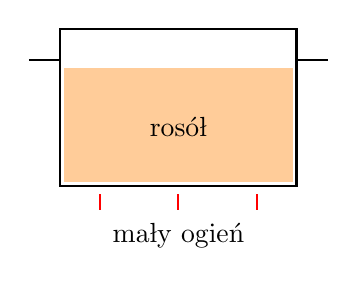
\begin{tikzpicture}
    \draw[thick] (0,0) rectangle (3,2);
    \draw[thick] (-0.4,1.6) -- (0,1.6);
    \draw[thick] (3,1.6) -- (3.4,1.6);
    \fill[orange!40] (0.05,0.05) rectangle (2.95,1.5);
    \node at (1.5,0.75) {rosół};
    \foreach \x in {0.5,1.5,2.5} \draw[red, thick] (\x,-0.3) -- (\x,-0.1);
    \node[below] at (1.5,-0.35) {mały ogień};
  \end{tikzpicture}
  \caption{Garnek z rosołem na małym ogniu}
  \label{fig:pot}
\end{figure}

\section{Czas gotowania}
\label{sec:time}

Czas gotowania $t$ (w godzinach) zależy od masy mięsa $m$ (w kilogramach) i wyraża się wzorem
\begin{equation}
  t = 1{,}5 + 0{,}6 \cdot m ,
  \label{eq:time}
\end{equation}
co dla porcji z tabeli~\ref{tab:ingredients} daje $t = \num{2.4}$~h.
\supervisor{Skąd ten wzór? Brak źródła!}

\section{Automatyzacja}
\label{sec:automation}

Przeliczanie składników na inną liczbę porcji wykonuje funkcja \code{scale_recipe} z listingu~\ref{lst:scale}.
Kod wczytywany jest wprost z pliku, więc w dokumencie jest zawsze jego aktualna wersja.

\lstinputlisting[
  language=Python,
  caption={Przeliczanie składników (plik \texttt{scripts/scale\_recipe.py})},
  label={lst:scale},
]{scripts/scale_recipe.py}


\printbibliography[heading=bibintoc, title={Wykaz literatury}]
\listoffigures
\listoftables
\lstlistoflistings

\end{document}
